% I suggest we discuss briefly Timepix detectors use on the ISS and other places for space radiation dosimetry and particle identification. We can also talk a bit about our motivations of studying cosmic rays on commercial airline flights.
%
% Find model to fit our data
%
% Mention motivation for study, such as GCR's, seeing the Regener-Pfotzer Maximum, space flight and radiation importance, commercial air flights.  LOW COST RAPSBERRY PI SYSTEM.
%
\section{Background}
\label{Background}
%%% GCR's and Regener-Pfotzer Maxiumum, space flight ----- Work in Progress
Space radiation and galactic cosmic rays (GCRs) pose real health risks to astronauts and pilots in any field.  Radiation exposure in Low Earth Orbit and the atmosphere must be monitored to ensure they do not exceed the occupational dose limits.  The ability to measure real-time exposure is arguably a crucial tool that can help mitigate risks.  Studying radiation types and dose levels near the nebulous border between space and Earth's atmosphere, and within the various zones of the atmosphere, facilitates preparation for current and future space missions; and aviation in general.  
%No edits have been made after this point yet.
To monitor the radiation in the upper atmosphere and beyond, a USB TimePIX device could be effectively used as a low cost dosimeter.  TimePIX detectors have many applications in the realm of particle physics, specially with their small physical and power consumption footprint. Overall, TimePIX devices could be setup to create a network of devices to better understand the Earth space radiation environment and observe space weather.
%
%
%%%   Lets tie this together, actual space below
%
%
Numerous balloon flights have included the use of TimePIX devices for the purposes of particle imaging and radiation dosimetry in unusual and unfamiliar environments, such as the stratosphere \cite{bexus}. 
%
The International Space Station (ISS) uses TimePIX devices to evaluate the astronauts' exposure to ionizing radiation fields \cite{timepix}.
% below is an actual space

The TimePIX device used in this flight was a MiniPIX, which is a silicon-based hybrid pixel detector built by ADVACAM \cite{advacam}. 
%
The sensor surface offers a resolution of 256x256 pixels.
%
The device can be operated under one of three modes: time-of-arrival (TOA) or time-over-threshold (TOT), or single particle counting. 
%
%When a particle ionizes with the silicon chip, the deposited charge is depleted by a bias voltage in a process known as Carrier generation and recombination. \textbf{<<Verify the previous statement>>}
%I think we can simplify this statement into this, since we don't have to go too deep into the background.  Just the basics works.
When a charged particle interacts with the silicon chip, ionization currents are created which are detected and measured by the device.

\begin{figure}[h]
    \centering
    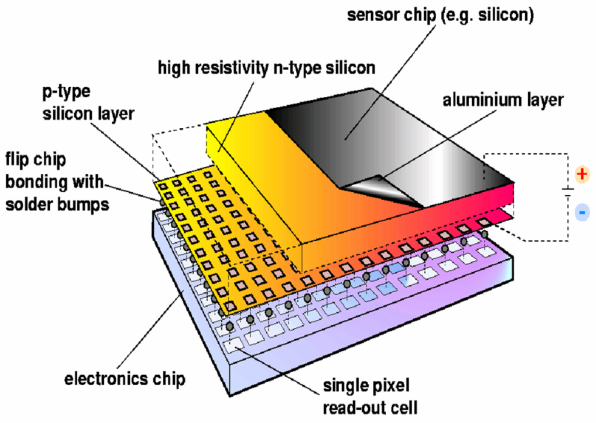
\includegraphics[width=0.35\textwidth]{minipix_silicon.pdf}
    \caption{MiniPIX silicon concept design}
    \label{fig:minipix_silicon}
\end{figure}
%
%figure name: minipix_silicon.pdf
%

%This was copied over to the "Experiment Design Section"
%For the SORA flights, the MiniPIX was coupled with a low cost open ARM based computer.  Both flights utilized a Raspberry Pi 3 to communicate and handle all operations with the MiniPIX.  This system allowed for remote operation and on-board analyzation of all data.  The SORA flights tested the feasibility of these low-cost systems to fly further space missions.  